\documentclass[../../diss.tex]{subfiles}
\begin{document}

\section{Valence systems over graph monoids}%
\label{Valence:Systems}

In this section, we will formally introduce the model of valence systems over graph monoids~\cite{Zetzsche15d} that we will use in the rest of this chapter.

\paragraph{Valence systems}

Recall that a \emph{monoid} is a tuple $(\monoid,\cdot,\neutral)$ where $\monoid$ is a non-empty set and $\cdot \ \colon \monoid \times \monoid \to \monoid$ is a binary operation on $\monoid$ that satisfies \emph{associativity}, \ie $x \cdot (y \cdot z) = (x \cdot y) \cdot z$ holds for all $x,y,z \in \monoid$.
Furthermore, $\neutral \in \monoid$ is neutral with respect to the operation, $x \cdot \neutral = \neutral \cdot x = x$ for all $x \in \monoid$.
In the following, we will usually say that a set $\monoid$ is a monoid and assume that the operation and the neutral element are clear from the context.

A set of \emph{generators} of a monoid $\monoid$ is a subset $G \subseteq \monoid$ such that all elements of $\monoid$ can be obtained by iteratively composing elements of $G$.
A monoid is \emph{finitely generated} if it has a finite set of generators.
%
For example, consider the monoid $(\N,+,0)$, the natural numbers with addition.
It is generated by the set $\set{1}$: Zero is obtained as the empty composition (which always yields the neutral element), and every other number can be obtained by adding up $1$ \nb{suitably often}.

A \emph{valence system} over monoid $\monoid$ is an automaton with finitely many control states that uses the elements of the monoid $\monoid$ as storage.
Syntactically, it is a finite-state LTS with monoid elements as transition labels.
Its semantics is defined as follows:
A configuration is of the shape $(q,m)$, consisting of a control state $q$ and a monoid element $m \in \monoid$.
A transition $q \tow{m'} q'$ that originates in control state $q$ can be applied to this configuration, leading to the new configuration $(q, m \cdot m')$.
%
This means that monoid elements represent both storage values and operations on the storage:
The monoid element $m'$ induces the operation $\cdot m'$ that composes the current storage value with $m'$.
The neutral element represents the empty storage \resp the operation that does not modify the storage.

For the reachability problem for valence systems, we assume that a unique initial and a unique final control state, $q_\init$ and $q_\final$, have been fixed.
The goal is to reach the final state with empty storage starting from the initial state with empty storage.

\begin{problem}
    \problemtitle{Reachability for valence systems}
    \probleminput{Valence system over some monoid $\monoid$.}
    \problemquestion{$(q_\init,\neutral) \to^* (q_\final,\neutral)$?}
\end{problem}

The definition of the reachability problem justifies the right-invertibility restriction that we introduce in the following.
A monoid element $m$ is called \emph{right invertible} if it has a right inverse, a monoid element $m'$ such that $m \cdot m' = \neutral$.
It is clear that it is only possible to reach $(q_\final,\neutral)$ from some configuration $(q,m)$ if $m$ is right invertible -- right invertibility is a necessary condition.
This allows us to forbid transitions that would lead to a storage value that is not right invertible without altering the answer to the reachability problem.

Altogether, we obtain the following formal definition of valence systems and their semantics.

\begin{definition}
    Syntactically, a \emph{valence system} is \( \lts = (\monoid, Q, \delta, \qinit, \qfinal) \)
    where $\monoid$ is a monoid, $Q$ is a finite set of states, $\qinit, \qfinal \in Q$ and $\delta \subseteq Q \times \monoid \times Q$.
    Its semantics is the induced transition system whose configurations are from the set $Q \times \monoid$.
    % with the initial configuration being $(\qinit,\neutral)$.
    The transition relation $\delta$ induces a transition relation among configurations: $(q,m) \to (q'',m'')$ if there is a transition $q \tow{m'} q''$ in $\delta$ such that $m'' = m \cdot m'$ and $m''$ is right invertible.
\end{definition}

It is straightforward to define valence automata as versions of valence system in which transitions are additionally labeled by letters from a finite alphabet.
We can associate to the computations that are witnesses for reachability the finite words that occur as their labels, and hence obtain a definition for the language of a valence automaton.

Whether the reachability problem (and other problems for valence systems and automata) can be solved algorithmically depends on the underlying monoid.
We will see later that there is a fixed monoid such that the class of valence system over that monoid is Turing-complete and hence the reachability problem is undecidable.
The main goal of the research on valence systems is to classify the monoids for which certain problems are solvable.

However, the class of all monoids turns out to be too diverse to be able to obtain such classification results.
There is a lack of criteria that are expressible on the level of general monoids that would be needed for a classification.
There are two subclasses that come to mind as candidates on which one could base a classification.
The first is the class of all finitely generated monoids.
However, this class is still too diverse.
In fact, since a valence system has a finite number of transitions, also the number of distinct transition labels is finite.
The set of all reachable storage values is contained in the submonoid that is generated by these transition labels.
In short, the restriction to finitely generated monoids is not a restriction at all.
%
The second subclass that comes to mind is the class of all finite monoids.
It is easy to see, however, that the class of valence systems over such monoids is just as expressive as the class of finite-state systems without any storage.
The transition system induced by such a valence system would again be finite state.

\paragraph{Graph monoids}

In the following, the class of graph monoids~\cite{Zetzsche15d,Charney07} will serve as a basis for our classification results.
It is a class of potentially infinite monoids, each of which can be described by a finite undirected graph.\footnote{Note the analogy to automata theory, where we are interested in systems with a potentially infinite semantics that admit a finite syntactic representation.}

We consider graphs $G = (V,\indep)$ where $V$ is a finite set of nodes, and the edges are given by $\indep \subseteq V \times V$, the \emph{independence relation}.
The latter is symmetric, \ie $o_1 \indeprel o_2$ implies $o_2 \indeprel o_1$.
It is neither necessarily reflexive nor necessarily anti-reflexive; $o_1 \indeprel o_1$ only holds if the graph has a self-loop at node $o_1$.
We use infix notation and write $o_1 \indeprel o_2$ for $(o_1, o_2) \in \indep$ and $o_1 \notindeprel o_2$ \nb{for $(o_1,o_2) \not\in \indep$}.

Intuitively, the nodes of $V$ are parts of the storage, and the independence relation specifies which parts of the storage are independent of each other.
The graph monoid induced by such a graph consists of all sequences of storage operation, where we identify sequences that are equal but for the order of actions on independent parts of the storage.
More formally, we associate to each node $o \in V$ two operations, a positive operation $\inc{o}$ (\enquote{push~$o$}, \enquote{increment~$o$}) and a negative operation $\dec{o}$ (\enquote{pop~$o$}, \enquote{decrement~$o$}).
We call $+$ \resp $-$ the polarity of the operation.
By $\incdec{o}$ we denote an arbitrary element from $\set{ \inc{o}, \dec{o}}$.
Let $\ops = \Set{ \inc{o}, \dec{o} }{ o \in V }$ denote the set of all operations.
We start by considering the free monoid $\ops^*$ over $\ops$, \ie the set of all finite-length sequences over $\ops$ with concatenation as the operation and the empty sequence~$\eps$ as the neutral element.
To obtain the \emph{graph monoid $\graphmonoid = \ops^* /_{\cong}$ for graph $G$}, we factorize $\ops^*$ by the smallest congruence $\cong$ (with respect to concatenation) that satisfies
\begin{align}
    \label{Rule:Cancel}\tag{G1}
        \inc{o}.\dec{o} &\cong \eps
        \quad\quad\quad\hspace*{0.7em} \text{ for all } o \in V
        \text{, and}
        \\
    \label{Rule:Swap}\tag{G2}
        \incdec{o_1}.\incdec{o_2} &\cong \incdec{o_2}.\incdec{o_1}
        \quad \text{ for all } o_1 \indeprel o_2
        \ .
\end{align}
Intuitively, the first rule states that $\dec{o}$ is the right inverse of $\inc{o}$ -- an increment followed by a decrement leaves the storage unchanged.
The second rule formalizes the above-mentioned intuition that sequences that differ only in the order of independent actions (actions $\incdec{o_1},\incdec{o_2}$ with $o_1 \indeprel o_2$) should be identified.

Elements of the graph monoid are congruence classes of sequences over $\ops$ \wrt $\cong$.
The operation of the monoid can be applied by concatenating representatives of classes.
The neutral element is the equivalence class of the empty word $\eps$.
It represents the empty storage, and concatenating it is the operation that leaves the storage unchanged.
We will often use sequences to denote monoid elements and extend the corresponding notations and definitions whenever there is no risk of causing ambiguity.

\begin{remark}%
\label{Remark:ValenceSelfLoops}%
    We briefly discuss the implications of a node having or not having a self-loop in the graph.

    If node $o_1$ does not have a self-loop, $o_1 \notindeprel o_1$, then the negative operation $\dec{o}$ is not the right inverse of the positive operation $\inc{o}$.
    \RuleCancel only applies to the sequence $\inc{o}.\dec{o}$, not to $\dec{o}.\inc{o}$.
    In fact, $\dec{o}$ is not right invertible in this case.

    If $o_1$ has a self-loop, $o_1 \indeprel o_1$, then $\dec{o}$ is the right inverse of $\inc{o}$.
    We can first apply \RuleSwap to obtain $\dec{o}.\inc{o} \cong \inc{o}.\dec{o}$, and then cancel the two operations using \RuleCancel.
\end{remark}

In the following, we will speak of a valence system over a graph and mean the valence system over the graph monoid defined by that graph.
We will also call the underlying graph the \emph{storage graph} of the system for obvious reasons.

Before giving some examples, we will need the notion of an induced subgraph.

\begin{definition}
    For a graph $G = (V,\indep)$ and a set of nodes $V' \subseteq V$, the \emph{subgraph induced by $V'$} is the graph $(V', \indep \cap (V' \times V'))$, \ie the graph that is obtained from $G$ by discarding all nodes not in $V'$ and all edges involving discarded nodes.
\end{definition}

A graph is an \emph{induced subgraph} of $G$ if it occurs as the subgraph induced by a suitable set of nodes.
Unlike normal subgraphs, induced subgraphs do not allow us to discard arbitrary edges.
If a graph contains an edge, then any induced subgraph that contains the nodes connected by the edge will also contain that edge.

The expressiveness of valence systems is monotonic with respect to the subgraph order:
The class of valence system over some graph $G$ is at least as expressive as the class of valence system over any subgraph of $G$.

The class of graph monoids is a good basis for a classification of valence systems with respect to their algorithmic properties.
On the one hand, graph-theoretic properties like connectedness are related to the decidability of certain problems for the valence systems over the corresponding graph monoids.
On the other hand, valence systems over graph monoids generalize many well-known models of computation.
This means that various types of automata will fit into the classification.
We demonstrate this in the form of a few examples.
We refer to Chapter~2.9 of~\cite{Zetzsche15d} for more details.

\begin{figure}[t]
    {\centering\subcaptionbox{pushdown systems.\label{Figure:ValenceSystemExamplesPDS}}[0.24\textwidth][c]{
        \begin{tikzpicture}[->,>=latex,node distance=1em,semithick]

\node (a) at (0,0) {$\bullet$};
\node (b) at (1,0) {$\bullet$};

\node at (0.5,-0.4) {};

\node [left of=a] {$a$};
\node [right of=b] {$b$};

\end{tikzpicture}
}
    }
    {\centering\subcaptionbox{multi-pushdown systems.\label{Figure:ValenceSystemExamplesMPDS}}[0.24\textwidth][c]{
        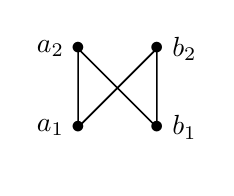
\begin{tikzpicture}[->,>=latex,node distance=1em,semithick]

\node (a) at (0,0) {$\bullet$};
\node (b) at (1,0) {$\bullet$};
\node (a2) at (0,1) {$\bullet$};
\node (b2) at (1,1) {$\bullet$};

\node at (0.5,-0.4) {};

\node [left of=a] {$a_1$};
\node [right of=b] {$b_1$};
\node [left of=a2] {$a_2$};
\node [right of=b2] {$b_2$};

\path [draw,-]
    (a.center) -- (a2.center)
    (a.center) -- (b2.center)
    (b.center) -- (a2.center)
    (b.center) -- (b2.center)
;

\end{tikzpicture}
}
    }
    {\centering\subcaptionbox{VASSes / Petri nets.\label{Figure:ValenceSystemExamplesVASS}}[0.24\textwidth][c]{
        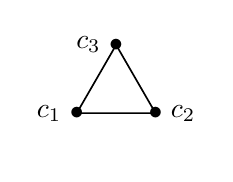
\begin{tikzpicture}[->,>=latex,node distance=1em,semithick]

\node (a) at (0,0) {$\bullet$};
\node (b) at (1,0) {$\bullet$};
\node (c) at (60:1) {$\bullet$};

\node at (0.5,-0.4) {};

\node [left of=a] {$c_1$};
\node [right of=b] {$c_2$};
\node [left of=c] {$c_3$};

\path [draw,-]
    (a.center) -- (b.center)
    (a.center) -- (c.center)
    (b.center) -- (c.center)
;

\end{tikzpicture}
}
    }
    {\centering\subcaptionbox{integer VASSes / integer Petri nets.\label{Figure:ValenceSystemExamplesIntegerVASS}}[0.24\textwidth][c]{
        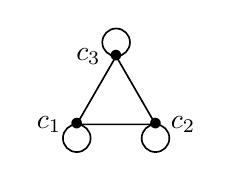
\begin{tikzpicture}[->,>=latex,node distance=1em,semithick]

\node (a) at (0,0) {$\bullet$};
\node (b) at (1,0) {$\bullet$};
\node (c) at (60:1) {$\bullet$};

\node [left of=a] {$c_1$};
\node [right of=b] {$c_2$};
\node [left of=c] {$c_3$};

\node at (0.5,-0.4) {};

\path [draw,-]
    (a.center) -- (b.center)
    (a.center) -- (c.center)
    (b.center) -- (c.center)
;

\draw (a.center) ++(-90:0.5em) circle (0.5em);
\draw (b.center) ++(-90:0.5em) circle (0.5em);
\draw (c.center) ++(90:0.5em) circle (0.5em);

\end{tikzpicture}
}
    }
    \caption{Graphs for which valence systems over the corresponding graph monoids are \ldots}%
    \label{Figure:ValenceSystemExamples}%
\end{figure}

\begin{example}%
\label{Example:ValenceSystemExamples}%
    \begin{thmenumerate}[a)]
        \item
            The empty graph induces the graph monoid with $\eps$ as the single element.
            Valence systems over this graph are finite-state systems, and any finite state system can be seen a valence system over this graph.
        \item
            Consider the graph with two nodes $a$ and $b$ and no edge, \ie the empty independence relation.
            It is depicted in \cref{Figure:ValenceSystemExamplesPDS}.
%
            As observed in \cref{Remark:ValenceSelfLoops}, neither $\dec{a}$ nor $\dec{b}$ are right invertible.
            In fact, any right-invertible element of the monoid can be represented by a sequence over $\set{ \inc{a}, \inc{b} }$ that exclusively uses the positive operations, and any such sequence represents a unique element of the graph monoid.
            Any sequence involving a negative operation, \eg $\dec{a}$, can only represent a right-invertible monoid element if it contains an earlier occurrence of $\inc{a}$ such that the two cancel out.

            The right-invertible elements of the graph monoid over are the configurations of a LIFO stack (last in, first out) over the stack alphabet $\set{a,b}$.
            The operation $\cdot \inc{a}$ pushes $a$ onto the stack, the operation $\cdot \dec{a}$ removes $a$ from the top of the stack.
            The latter can only be applied if the current storage value can be represented by a sequence whose last element is $\inc{a}$; otherwise, we end up with a value that is not right invertible.

            With this reasoning, a valence system over this graph is a pushdown system with a binary stack alphabet as introduced in \cref{Section:CFG}.
            A pushdown system with a $k$-letter stack alphabet can be seen as a valence system over a graph with $k$ unconnected nodes that have no self-loops.
        \item
            Consider the graph with nodes ${a_1,b_1,a_2,b_2}$ and the edges $a_1 \indeprel a_2$, $a_1 \indeprel b_2$, $b_1 \indeprel a_2$, $b_1 \indeprel b_2$ (and their symmetric versions).
            It is depicted in \cref{Figure:ValenceSystemExamplesMPDS}.
            Note that the subgraphs induced by both $\set{a_1,b_1}$ and $\set{a_2,b_2}$ are the graph that we considered in Part~b).
            Furthermore, each node $x_1$ is connected to each node $y_2$ for $x,y \in \set{a,b}$.

            The right-invertible elements of the corresponding graph monoid can be represented by sequences of the shape $w_1.w_2$ where $w_1$ exclusively contains the positive operations over $\set{\inc{a_1}, \inc{b_1}}$, similar for $w_2$ and $\set{\inc{a_2}, \inc{b_2}}$.
            Given an arbitrary representative, we first use \RuleSwap~to reorder it into a prefix containing the operations corresponding to $\set{a_1,b_1}$ and a suffix.
            Then, we proceed as in Part~b) of the example and use \RuleSwap~exhaustively to remove occurrences of negative operations.
            If a negative operation cannot be removed, the sequence does not represent a right-invertible monoid element.

            The right-invertible elements of the graph monoid represent configurations of two independent LIFO stacks, each over a binary stack alphabet.
            Hence, the corresponding valence systems are multi-pushdown systems that use such stacks as storage.
            It is well-known that multi-pushdown systems with at least two stacks and at least two symbols on each stack are Turing-complete:
            Intuitively, each of the stacks can store one half of the tape content of a Turing machine.
            Rice's theorem~\cite{Rice53} applies and all non-trivial semantic properties of valence systems over this graph monoid are undecidable.
        \item
            Consider a 3-clique with no self-loops, \ie a graph with the set of nodes $\set{c_1,c_2,c_3}$ in which any two distinct nodes are connected by an edge.
            It is depicted in \cref{Figure:ValenceSystemExamplesVASS}.

            Every right-invertible element of the corresponding graph monoid can be represented by a sequence of the shape ${(\inc{c_1})}^{n_1}{(\inc{c_2})}^{n_2}{(\inc{c_2})}^{n_3}$.
            Hence, these elements represent tuples $(n_1,n_2,n_3) \in \N^3$ of counter values and the positive and negative operation for each $c_i$ increment and decrement the corresponding counter value $n_i$, respectively.
            The decrement is blocking, it can only be applied if the corresponding component is non-zero; otherwise, we end up with a value that is not right invertible.
            One also says that the nodes of the storage graph are \emph{partially blind counters}:
            Their value cannot be tested for being zero during runtime, but non-zeroness can be asserted by using the blocking decrement.

            Valence systems over this graph are $3$-dimensional vector addition systems with states (VASSes), a model that we have mentioned in \cref{Section:PNUnlabeled} as being equivalent to Petri nets with a corresponding number of unbounded places.
            VASSes of arbitrary dimension $k$ can be seen as valence systems over a $k$-clique with no self-loops.
        \item
            We add a self-loops to every node of the graph from Part~d).
            The result is depicted in \cref{Figure:ValenceSystemExamplesIntegerVASS}.

            The self-loops mean that \eg $\inc{c_1}$ is now the right inverse of $\dec{c_1}$ in the graph monoid:
            We can first use \RuleSwap~to swap them, then use \RuleCancel~to cancel them out.
            More precisely, every element of the graph monoid is right invertible.
            It represents a tuple of counters $(n_1,n_2,n_3) \in \Z^3$ that may attain negative values.
            Since we have no blocking decrement at hand to assert non-zeroness during runtime, we call these counters \emph{blind}.

            Valence systems over such graph monoids are integer vector addition systems with states, a model that corresponds to integer Petri nets or Petri nets that work on pseudo-markings, see \cref{Section:PNUC}.
    \end{thmenumerate}

    In addition to these well-known types of automata, valence systems can also model various other interesting types of storage.
    This includes automata that use a stack of counters as storage, and automata that have access to both a stack and a set of partially blind counters.
    The latter model is sometimes called a \emph{pushdown Petri net (PPN)}; it is famous for the fact that the decidability status of its reachability problem is a long-standing open question, see \eg~\cite{Lazic13}.
    One such \emph{PPN graph} is depicted in \cref{Figure:ValenceSystemExamplesPPN}.
    It consists of a stack with two stack symbols $a, b$ and a partially blind counter $c$ that is independent of both $a$ and $b$.
\end{example}

\begin{figure}[t]
    \centering%
    {%
        \centering%
        \subcaptionbox{The graph $P_4$.\label{Figure:ValenceSystemExamplesC4}}[0.4\textwidth][c]%
        {%
            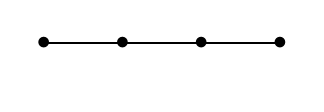
\begin{tikzpicture}[->,>=latex,node distance=1em,semithick]

\node (a) at (0,0) {$\bullet$};
\node (b) at (1,0) {$\bullet$};
\node (c) at (2,0) {$\bullet$};
\node (d) at (3,0) {$\bullet$};

\node at (0.5,-0.4) {};


\path [draw,-]
    (a.center) -- (b.center)
    (b.center) -- (c.center)
    (c.center) -- (d.center)
;


\end{tikzpicture}
%
        }%
    }%
    {%
        \centering%
        \subcaptionbox{The graph $C_4$.\label{Figure:ValenceSystemExamplesP4}}[0.3\textwidth][c]
        {%
            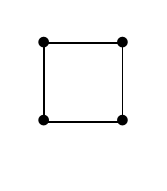
\begin{tikzpicture}[->,>=latex,node distance=1em,semithick]

\node (a) at (0,0) {$\bullet$};
\node (b) at (1,0) {$\bullet$};
\node (a2) at (0,1) {$\bullet$};
\node (b2) at (1,1) {$\bullet$};

\node at (0.5,-0.4) {};

\path [draw,-]
    (a.center) -- (a2.center)
    (b.center) -- (b2.center)
    (a.center) -- (b.center)
    (a2.center) -- (b2.center)
;

\end{tikzpicture}
%
        }%
    }%
    {%
        \centering%
        \subcaptionbox{A PPN graph.\label{Figure:ValenceSystemExamplesPPN}}[0.3\textwidth][c]
        {%
            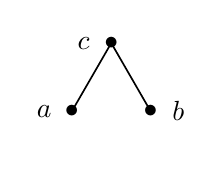
\begin{tikzpicture}[->,>=latex,node distance=1em,semithick]

\node (a) at (0,0) {$\bullet$};
\node (b) at (1,0) {$\bullet$};
\node (c) at (60:1) {$\bullet$};

\node at (0.5,-0.4) {};

\node [left of=a] {$a$};
\node [right of=b] {$b$};
\node [left of=c] {$c$};

\path [draw,-]
    (a.center) -- (c.center)
    (b.center) -- (c.center)
;

\end{tikzpicture}
%
        }%
    }%
    \caption{Graphs for which reachability in valence systems is undecidable, or not known to be decidable in the case of c).}%
    \label{Figure:ValenceSystemExamplesEvil}%
\end{figure}

Valence systems over graph monoids cannot model all types of automata models.
For example, they can neither model higher-order systems as defined in \cref{Section:HORS}, nor FIFO (first in, first out) queues.
For a detailed explanation why modelling queues is impossible, we refer to Section~2 of our publication~\cite{MeyerMZ18}.

Georg~Zetzsche has provided a classification of the decidability of the reachability problem for valence systems over graph monoids~\cite{Zetzsche15c}.
For the sake of simplicity, we restrict ourselves to graphs with no self-loops in the following.
Let $C_4$ denote a cycle of four nodes, and let $P_4$ be a path of four nodes.
These graphs are depicted in \cref{Figure:ValenceSystemExamplesC4} and \cref{Figure:ValenceSystemExamplesP4}, respectively.
Note that the graph $C_4$ is equal to the graph from Part~c) of \cref{Example:ValenceSystemExamples} \resp \cref{Figure:ValenceSystemExamplesMPDS} that corresponds to multi-pushdown systems.
Zetzsche has shown that if a graph~$G$ contains $C_4$ or $P_4$ as an induced subgraph, then the reachability problem for valence systems over $G$ is undecidable.

The converse result is true if one excludes graphs that do correspond to the aforementioned pushdown Petri nets: If a graph neither contains $C_4$, nor $P_4$, nor one of several so-called PPN-graphs as an induced subgraph, then the reachability problem for valence systems over that graph is decidable.

Other classification results for valence systems and automata over graph monoids have been obtained in the literature, including classifications of the eliminability of silent transitions~\cite{Zetzsche13}, the context-freeness and the semi-linearity of the Parikh image of their languages~\cite{BuckheisterZ13}, and the decidability of first-order logic with reachability~\cite{DOsualdoMZ16}.

\end{document}
